\renewcommand{\theequation}{\theenumi}
\renewcommand{\thefigure}{\theenumi}
\begin{enumerate}[label=\thesubsection.\arabic*.,ref=\thesubsection.\theenumi]
\numberwithin{equation}{enumi}
\numberwithin{figure}{enumi}


\item Write down the equation of the tangent to a circle passing through the point $\vec{p}$. 

Equation of the circle and positional vector $\vec{p}$ is given as :
\begin{align}
    x^2+y^2-3x+10y&=15\label{eq:solutions/18/1/eq:0}\\
    \vec{p}&=\myvec{4\\-11}
\end{align}
\solution


General equation of the circle in vector form is :
\begin{align}
\vec{x}^T\vec{x}+2\vec{u}^T\vec{x}+f=0\label{eq:solutions/18/1/eq:1}
\end{align}
In the vector form \eqref{eq:solutions/18/1/eq:0} can be written as :
\begin{align}
\vec{x}^T\vec{x}+2\myvec{\frac{-3}{2}\\[0.1 cm]5}^T\vec{x}-15=0\label{eq:solutions/18/1/eq:2}
\end{align}
By comparing \eqref{eq:solutions/18/1/eq:1} and \eqref{eq:solutions/18/1/eq:2} we get : 
\begin{align}
    \vec{u}=\myvec{-\frac{3}{2}\\[0.1 cm]5},f=-15\label{eq:solutions/18/1/eq:3}
\end{align}
We know that the equation of tangent in the form of normal vector $(\vec{p}+\vec{u})$ and point $\vec{p}$ can be written as:
\begin{align}
    (\vec{p}+\vec{u})^T(\vec{x}-\vec{p})&=0\\
    (\vec{p}+\vec{u})^T\vec{x}-\vec{p}^T\vec{p}-\vec{u}^T\vec{q}&=0\label{eq:solutions/18/1/eq:5}
\end{align}
Using \eqref{eq:solutions/18/1/eq:1}, \eqref{eq:solutions/18/1/eq:5} will become : 
\begin{align}
    (\vec{p}+\vec{u})^T\vec{x}+\vec{u}^T\vec{p}+f&=0\label{eq:solutions/18/1/eq:6}
\end{align}
By putting the values of $\vec{p}$, $\vec{u}$ and $f$ from \eqref{eq:solutions/18/1/eq:3} in \eqref{eq:solutions/18/1/eq:6} we get : 
\begin{align}
    \myvec{\frac{5}{2}&-6}\vec{x}+\myvec{4&-11}\myvec{\frac{-3}{2}\\[0.2cm]5}-15&=0\\
    \myvec{\frac{5}{2}&-6}\vec{x}-76&=0
\end{align}
Hence the equation of the tangent to the circle passing through the point $\vec{p}$ is:
\begin{align}
    \myvec{\frac{5}{2}&-6}\vec{x}&=76\label{eq:solutions/18/1/eq:9}
\end{align}
Plot of the tangent to a circle given by equation \eqref{eq:solutions/18/1/eq:9} is as follows :
\begin{figure}[h]
\centering
    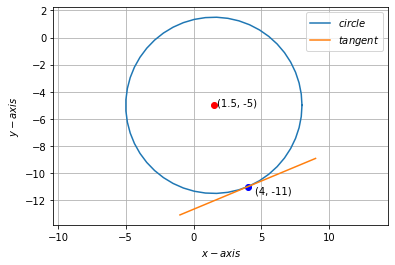
\includegraphics[width=\columnwidth]{solutions/18/1/tangent.png}
    \caption{Tangent to a circle centered at $(1.5, -5)$ with radius $6.5$ passing through the point $(4,-11)$.}
    \label{eq:solutions/18/1/tangent}
\end{figure}


\item Find equation of the tangent to the circle
\begin{align}
  x^2 + y^2 = 4 \label{eq:solutions/18/3/Latex/eq:1}
\end{align}
which is parallel to the line
\begin{align}
  x+2y-6=0  \label{eq:solutions/18/3/Latex/eq:2}
\end{align}
%
\solution
The equations for the circle and line in \eqref{eq:solutions/18/3/Latex/eq:1} and \eqref{eq:solutions/18/3/Latex/eq:2} can be rewritten in vector form as:
\begin{align}
  \norm{\vec{x}}^2 = 4 \\
  \myvec{1 & 2}\vec{x} = 6 \label{eq:solutions/18/3/Latex/eq:3}
\end{align}
The center of the circle happens to be $(0, 0)$ \\
The equation of a line is of the form:
\begin{align}
  \vec{n}^T\vec{x} = c \label{eq:solutions/18/3/Latex/eq:4}
\end{align}
Where n is the normal to the line. \\
Comparing \eqref{eq:solutions/18/3/Latex/eq:4} to \eqref{eq:solutions/18/3/Latex/eq:3},
\begin{align}
  \vec{n} = \myvec{1 \\ 2}
\end{align}
Since the tangent is parallel to the line in \eqref{eq:solutions/18/3/Latex/eq:3}, it will also have the same normal.

The point of contact for a conic is given by:
\begin{align}
  \vec{v} = \vec{V}^{-1}(\kappa\vec{n}-\vec{u}) \label{eq:solutions/18/3/Latex/eq:5}
\end{align}
where,
\begin{align}
  \kappa = \pm \sqrt[]{\frac{\vec{u}^T\vec{V^{-1}u}-f}{\vec{n}^T\vec{V}^{-1}\vec{n}}} \label{eq:solutions/18/3/Latex/eq:6}
\end{align}
For a circle,
\begin{align}
  \vec{V} = \vec{I}
\end{align}
Using properties of identity matrix, we get:
\begin{align}
  \vec{I}^{-1} = \vec{I} \\
  \vec{IX} = \vec{X}
\end{align}
Therefore \eqref{eq:solutions/18/3/Latex/eq:5} and \eqref{eq:solutions/18/3/Latex/eq:6} simplify to:
\begin{align}
  \kappa = \pm \sqrt[]{\frac{\vec{u}^T\vec{u}-f}{\vec{n}^T\vec{n}}} \\
  \implies \vec{v} = \kappa\vec{n-u}
\end{align}
Substituting the values, we get:
\begin{align}
  \kappa = \pm \sqrt[]{\frac{4}{\myvec{1 & 2}\myvec{1 \\ 2}}} \\
  \implies \kappa = \pm \sqrt[]{\frac{4}{5}} \\
  \vec{q} = \pm \sqrt[]{\frac{4}{5}}\myvec{1 \\ 2} \\
  \implies \vec{q_1} = \myvec{\sqrt[]{\frac{4}{5}} \\[0.2cm] \sqrt[]{\frac{16}{5}}}, \vec{q_2} = -\myvec{\sqrt[]{\frac{4}{5}} \\[0.2cm] \sqrt[]{\frac{16}{5}}}
\end{align}
Since there are two points of contact, there are two tangents parallel to \eqref{eq:solutions/18/3/Latex/eq:3} that have the same normal vector.
\begin{align}
  \implies \vec{n}^T\vec{q_1} = c_1 \\
  \vec{n}^T\vec{q_2} = c_2
\end{align}
Substituting the values, we get:
\begin{align}
  c_1 = 2\sqrt[]{5}, c_2 = -2\sqrt[]{5}
\end{align}
Therefore, the equation of the tangents are:
\begin{align}
  \myvec{1 & 2}\vec{x} = 2\sqrt[]{5} \\
  \myvec{1 & 2}\vec{x} = -2\sqrt[]{5}
\end{align}
The plot of the circle with the tangents is given below:
\begin{figure}[h]
\centering
    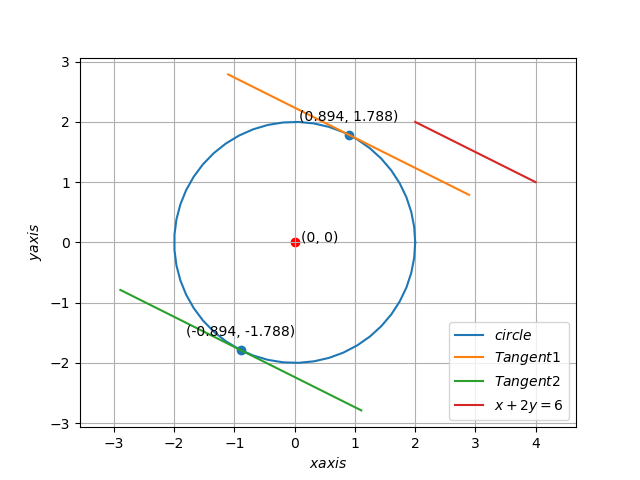
\includegraphics[width=\columnwidth]{solutions/18/3/Latex/Figure_1.png}
    \caption{Circle centered at $(0, 0)$ with tangents parallel to line $x+2y=6$.}
    \label{eq:solutions/18/3/Latex/fig:1}
\end{figure}

\end{enumerate}
